%-----------------------------------------------------------------------
% Cgcns : Compressible Navier Stokes Solver
% 
%           User Guide
%
%-----------------------------------------------------------------------
\documentclass{article}
% \usepackage[bookmarks=true]{hyperref} 
\usepackage[bookmarks=true,colorlinks=true,linkcolor=blue]{hyperref}

% \documentclass[xcolor=rgb,svgnames,dvipsnames,11pt]{article}
% \usepackage[bookmarks=true,colorlinks=true,linkcolor=blue]{hyperref}


% \input documentationPageSize.tex
\hbadness=10000 
\sloppy \hfuzz=30pt

% \voffset=-.25truein
% \hoffset=-1.25truein
% \setlength{\textwidth}{7in}      % page width
% \setlength{\textheight}{9.5in}    % page height

\usepackage{calc}
\usepackage[lmargin=.75in,rmargin=.75in,tmargin=.75in,bmargin=.75in]{geometry}

%- % set the page width and height for the paper (The covers will have their own size)
%- \setlength{\textwidth}{7in}  
%- \setlength{\textheight}{9.5in} 
%- % here we automatically compute the offsets in order to centre the page
%- \setlength{\oddsidemargin}{(\paperwidth-\textwidth)/2 - 1in}
%- % \setlength{\topmargin}{(\paperheight-\textheight -\headheight-\headsep-\footskip)/2 - 1in + .8in }
%- \setlength{\topmargin}{(\paperheight-\textheight -\headheight-\headsep-\footskip)/2 - 1in -.2in }

% \input homeHenshaw

\usepackage{amsmath}
\usepackage{amssymb}

\usepackage{verbatim}
\usepackage{moreverb}

\usepackage{graphics}    
\usepackage{epsfig}    
\usepackage{calc}
\usepackage{ifthen}
\usepackage{float}
% the next one cause the table of contents to disappear!
% * \usepackage{fancybox}

% \input{pstricks}\input{pst-node}
% \input{colours}

% define the clipFig commands:
% \input clipFig.tex
\usepackage{tikz}
\input ../common/trimFig.tex

\newcommand{\bogus}[1]{}  % begin a section that will not be printed

\usepackage{makeidx} % index
\makeindex
\newcommand{\Index}[1]{#1\index{#1}}


% ---- we have lemmas and theorems in this paper ----
\newtheorem{assumption}{Assumption}
\newtheorem{definition}{Definition}

% \newcommand{\docFigures}{\homeHenshaw/OvertureFigures}
% \newcommand{\figures}{\homeHenshaw/res/OverBlown/docFigures}
% \newcommand{\obFigures}{\homeHenshaw/res/OverBlown/docFigures}  % note: local version for OverBlown

\newcommand{\Overture}{{\bf Overture\ }}
\newcommand{\insDocDir}{../ins}
\newcommand{\cnsDocDir}{../cns}

% -------------  -------------------
\newcommand{\Solver}{Cgcns}
\newcommand{\solver}{cgcns}

% *** See http://www.eng.cam.ac.uk/help/tpl/textprocessing/squeeze.html
% By default, LaTeX doesn't like to fill more than 0.7 of a text page with tables and graphics, nor does it like too many figures per page. This behaviour can be changed by placing lines like the following before \begin{document}

\renewcommand\floatpagefraction{.9}
\renewcommand\topfraction{.9}
\renewcommand\bottomfraction{.9}
\renewcommand\textfraction{.1}   
\setcounter{totalnumber}{50}
\setcounter{topnumber}{50}
\setcounter{bottomnumber}{50}


% ***************************************************************************
\begin{document}


% -----definitions-----
\input ../common/wdhDefinitions.tex

\def\ud     {{    U}}
\def\pd     {{    P}}

\newcommand{\mbar}{\bar{m}}
\newcommand{\Rbar}{\bar{R}}
\newcommand{\Ru}{R_u}         % universal gas constant
\newcommand{\Div}{\grad\cdot}
\newcommand{\tauv}{\boldsymbol{\tau}}
\newcommand{\sumi}{\sum_{i=1}^n}
\newcommand{\dt}{{\Delta t}}

\vglue 5\baselineskip
\begin{flushleft}
{\Large
{\bf Cgcns} User Guide: An Overture Solver for the Compressible Navier--Stokes Equations on Composite Overlapping Grids,\\
}
\vspace{2\baselineskip}
William D. Henshaw,\\
Department of Mathematical Sciences, \\
Rensselaer Polytechnic Institute, \\
Troy, NY, USA, 12180.
\vspace{\baselineskip}
\today\\

\vspace{4\baselineskip}

\noindent{\bf\large Abstract:}

   Cgcns is a program that can be used to solve compressible fluid flow problems on overlapping
grids. It is built upon the \Overture object-oriented framework. 
Cgcns can be used to 
\begin{itemize}
  \item solve the compressible Navier--Stokes equations,
  \item solve the inviscid Euler equations with reactions, 
  \item solve problems on moving grids, 
  \item solve problems with adaptive mesh refinement.
\end{itemize} 

\end{flushleft}

\clearpage
\tableofcontents
% \listoffigures

\clearpage
\section{Introduction}

Cgcns is an compressible fluid flow solver for overlapping grids built upon
the \Overture framework~\cite{Brown97},\cite{Henshaw96a},\cite{iscope97}.
More information about
{\bf Overture} can be found on the \Overture home page, {\tt http://www.llnl.gov/\-casc/\-Overture}.


Cgcns can be used to 
\begin{itemize}
  \item solve the compressible Navier--Stokes equations,
  \item solve the inviscid Euler equations with reactions, 
  \item solve problems on moving grids, 
  \item solve problems with adaptive mesh refinement.
\end{itemize} 

The Cgcns solver is found in the {\tt cns} directory in the {\bf cg} distribution and has
sub-directories
\begin{description}
 \item[{\tt bin}] : contains the executable, cgcns. You may want to put this directory in your path.
 \item[{\tt check}] : contains regression tests.
 \item[{\tt cmd}] : sample command files for running cgcns, see section (\ref{sec:demo}).
%  \item[{\tt doc}] : dcoumentation.
 \item[{\tt lib}] : contains the Cgcns library, {\tt libCgcns.a}.
 \item[{\tt src}] : source files 
\end{description}


\noindent
Other documents of interest that are available through the \Overture home page are
\begin{itemize}
\item The Cgcns Reference Guide~\cite{CgcnsReferenceManual} for detailed descriptions of the
      equations, algorithms and discretizations.
\item The overlapping grid generator, {\tt Ogen}, \cite{OGEN}. Use this program to make grids for cgcns.
\item Mapping class documentation : {\ff mapping.tex}, \cite{MAPPINGS}. Many of the mappings that
   are used to create an overlapping grid are documented here. 
\item Interactive plotting : {\ff PlotStuff.tex}, \cite{PLOTSTUFF}.
\item {\tt Oges} overlapping grid equation solver, used by cgcns to solve implicit time stepping
    equations and the Poisson equation for the pressure, \cite{OGES}.
\end{itemize}

\subsection{Basic steps}\index{basic steps}
Here are the basic steps to solve a problem with Cgcns.
\begin{enumerate}
  \item Generate an overlapping grid with ogen. Make the grid with 2 ghost lines (this is the default).
  \item Run cgcns (note lowercase 'c', found in the {\tt bin/cgcns} directory) 
        and choose the PDE you want to solve.
  \item Assign the boundary conditions and initial conditions.
  \item Choose the parameters for the PDE (viscosity, reaction rates, ...)
  \item Choose run time parameters, time to integrate to, time stepping method etc.
  \item Compute the solution (optionally plotting the results as the code runs).
  \item When the code is finished you can look at the results (provided you saved a
     `show file') using {\tt plotStuff}.
\end{enumerate}
The commands that you enter to run cgcns can be saved in a \Index{command file} (by default
they are saved in the file `cgcns.cmd'). This command file can be used to re-run
the same problem by typing `cgcns file.cmd'. The command file can be edited to change parameters.

To get started you can run one of the demo's that come with cgcns, these are 
explained next in section~(\ref{sec:demo}).

Papers that describe some of the results obtained with Cgcns include~\cite{pog2008,mog2006,reactamr2003b}. 
  
\begin{figure}[hbt]
\begin{center}
  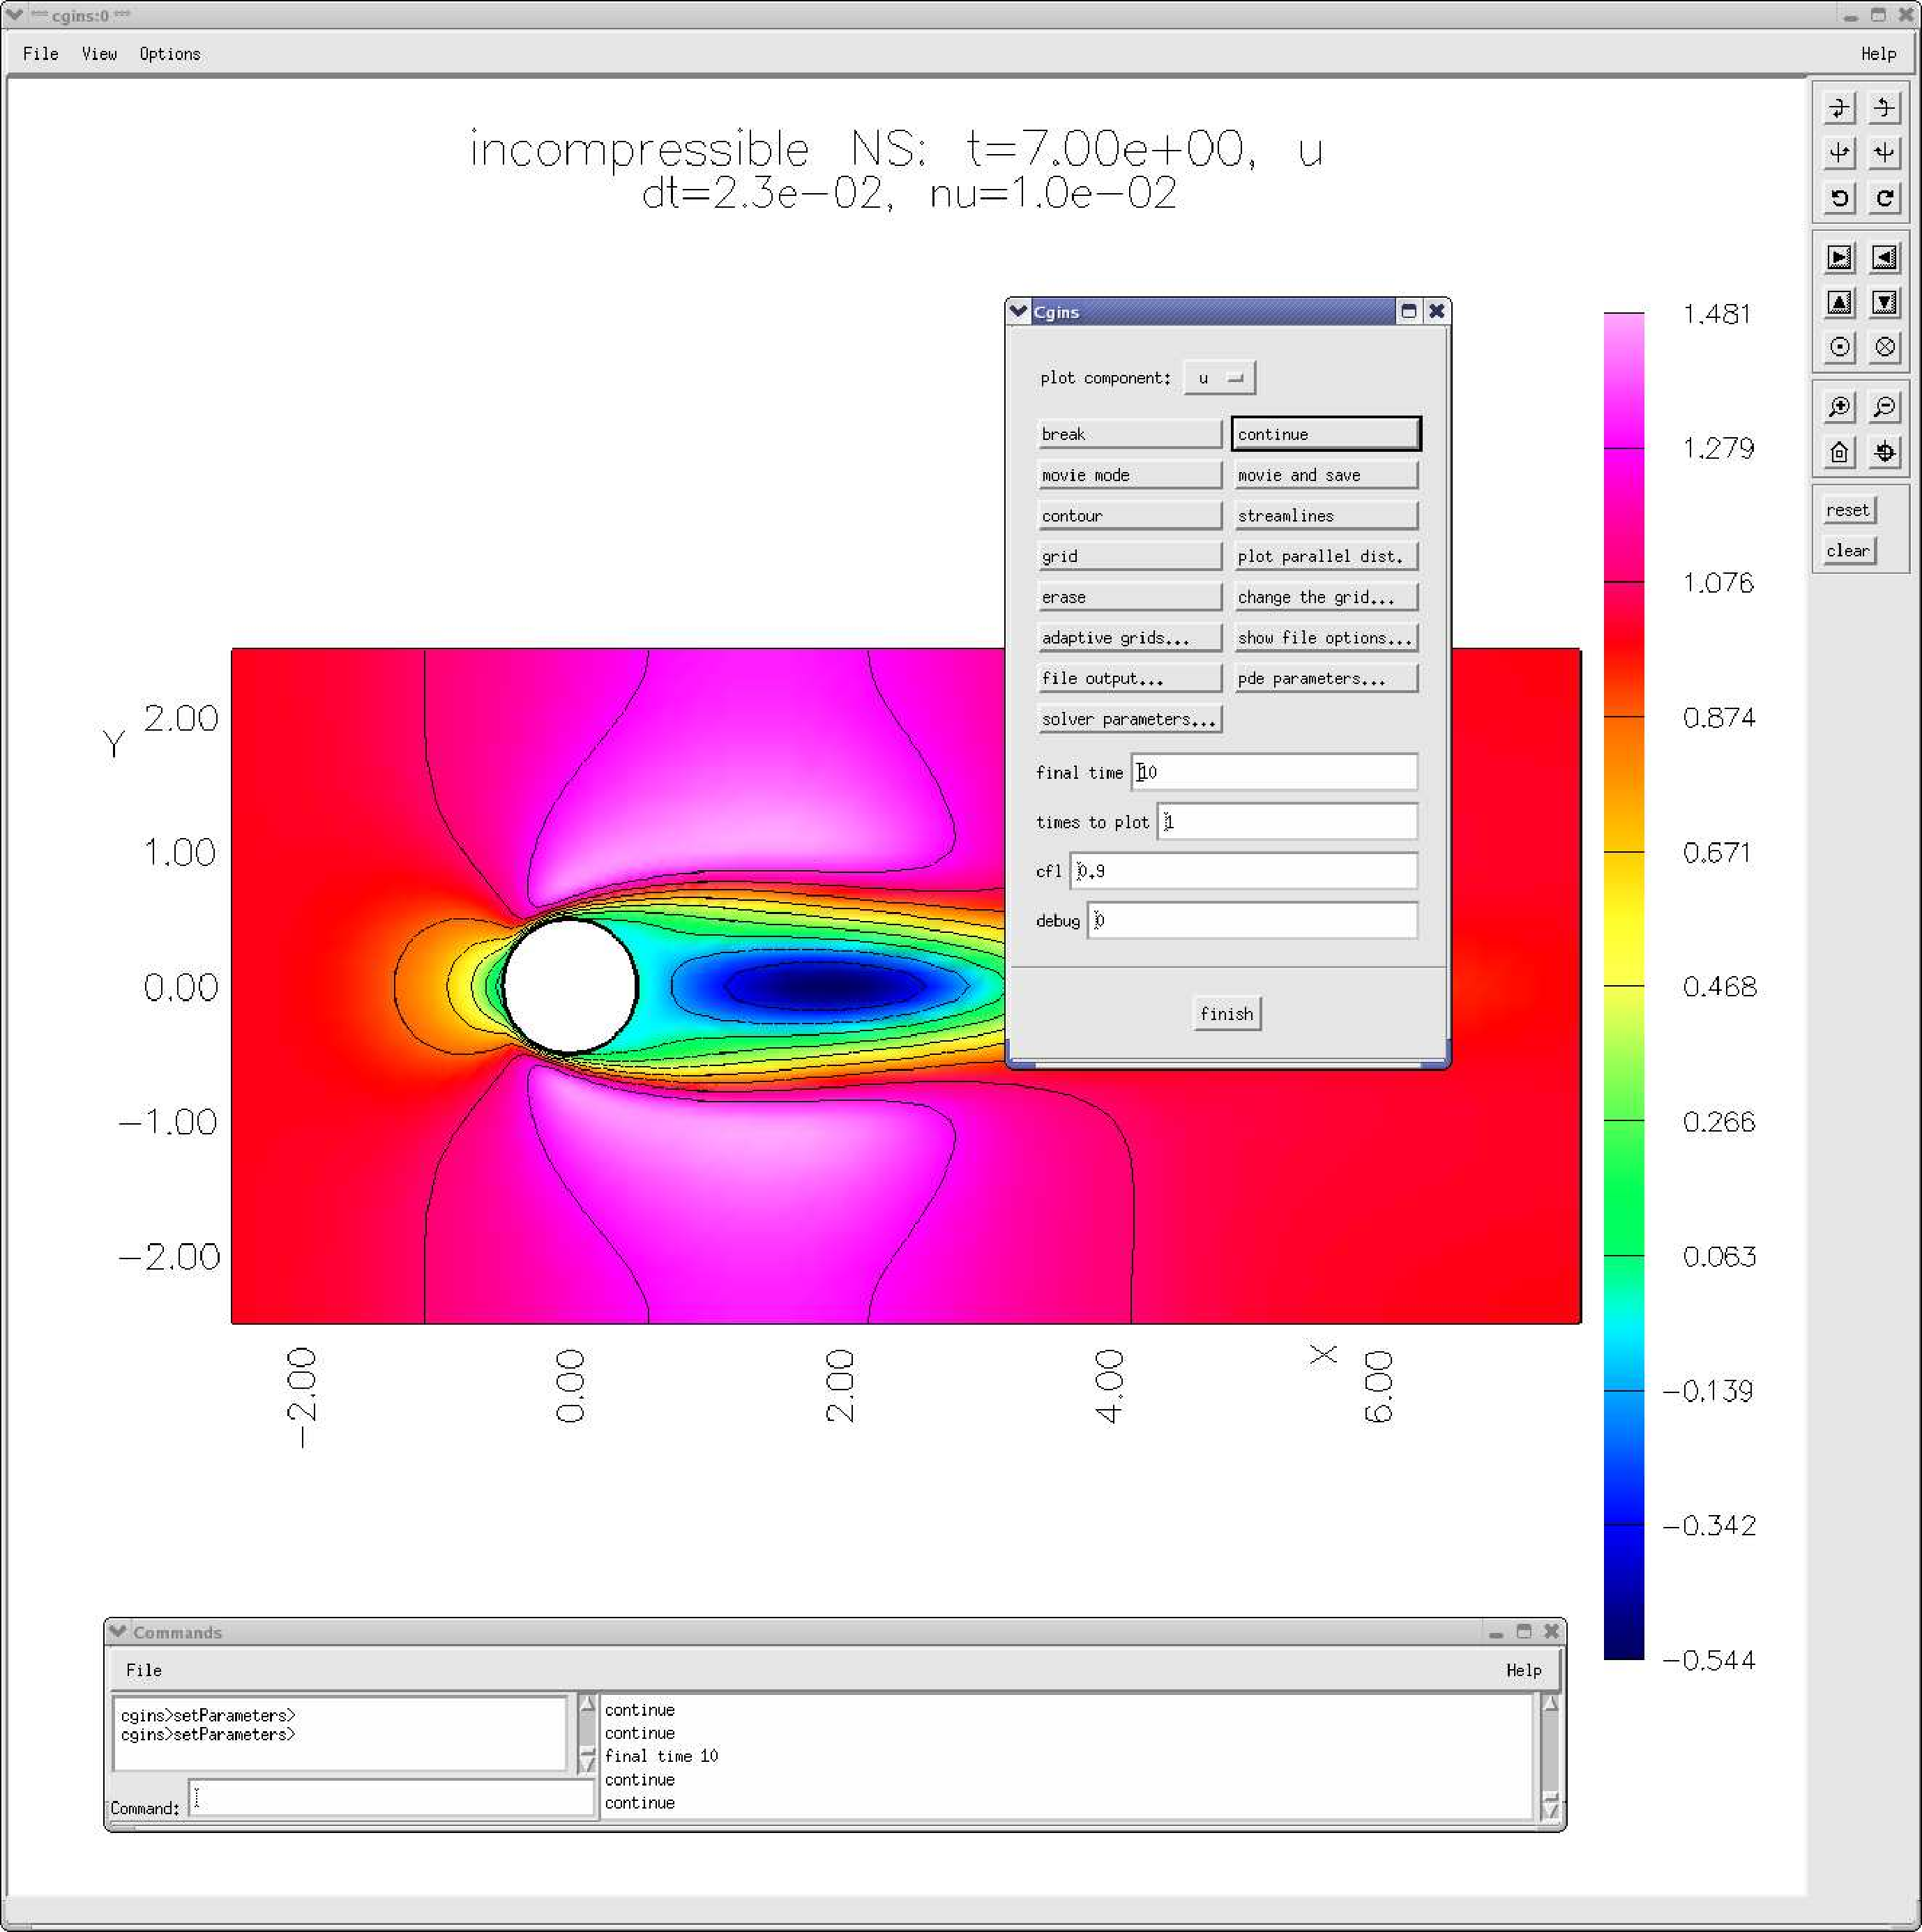
\includegraphics[width=.95\linewidth]{\insDocDir/cginsScreen} \\
  \caption{Snapshot of cgins (cgcns is similar) showing the run time dialog menu.}
  \end{center} 
  \label{fig:runTimeScreen}
\end{figure}



\clearpage
% ------------------------------------------------------------------------------------------------
\section{Sample command files for running cgcns} \label{sec:demo}

Command files are supported throughout the Overture. They are files
that contain lists of commands. These commands can initially be saved
when the user is interactively choosing options.  The \Index{command files}
can then be used to re-run the job. Command files can be edited and
changed.

In this section we present a number of command files that can be used
to run cgcns. See the file {\tt cg/cns/cmd/Readme} for a description of
the command files. 

% ------------------------------------------------------------------------------------------------
\subsection{Running a command file}

Given a \Index{command file} for cgcns such as {\tt cylinder.cmd}, found in {\tt
cmd/cylinder.cmd}, one can type `{\tt cgcns cylinder.cmd}' to run this command
file . You can also just type `{\tt cgcns cylinder}, leaving off the {\tt
.cmd} suffix. Typing `{\tt cgcns noplot cylinder}' will run without
interactive graphics (unless the command file turns on graphics). Note that here
I assume that the {\tt bin} directory is in your path so that the {\tt
cgcns} command is found when you type it's name. The Cgcns sample
command files will automatically look for an overlapping grid in the {\tt
Overture/sampleGrids} directory, unless the grid is first found in the location
specified in the command file.

When you run a command file a graphics screen will appear and after some
processing the run-time dialog should appear and the initial conditions will be
plotted. The program will also print out some information about the problem
being solved. At this point choose {\tt continue} or {\tt movie
mode}. Section~(\ref{sec:runTimeDialog}) describes the options available in the
run time dialog.

Many of the command files such as the stirring-stick problem, {\tt stir.cmd},
can take command line arguments.  For example, here
are two command lines that run a problem with different grids and parameters:
\begin{verbatim}
  cgcns stir -g=stir.hdf -nu=.05 -tf=1. -tp=.025 
  cgcns stir -g=stir2.hdf -nu=.01 -tf=1. -tp=.002 -rate=8.
\end{verbatim}
See the comments at the top of {\tt stir.cmd} for further explanation and examples.





% ------------------------------------------------------------------------------------------------
\clearpage
\subsection{Compressible flow past two offset cylinders}\index{compressible flow!two bumps}

This example demonstrates the method CNSCAD, solution of the compressible Navier-Stokes equations
using a conservative discretization with artificial diffusion.

The command file {\tt cg/cns/twoBump.cmd} can be used with \Solver to compute the
two-dimensional flow of a shock traveling past two offset cylinders. 
This example uses (a finer version) of the overlapping grid {\tt Overture/\-sampleGrids/\-twoBump.hdf}  generated
using the command file {\tt Overture/\-sampleGrids/\-twoBump.cmd}.
The coefficients of viscosity and heat conduction have been set to zero so that we
are solving the inviscid Euler equations.

{
\newcommand{\figWidth}{10cm}
\newcommand{\trimfig}[2]{\trimPlot{#1}{#2}{.12}{.15}{.35}{.325}}
\begin{figure}[hbt]
\begin{center}
\begin{tikzpicture}[scale=1]
  \useasboundingbox (0,.5) rectangle (10.,6.25);  % set the bounding box (so we have less surrounding white space)
%
  \draw ( 0.0,0.0) node[anchor=south west,xshift=-4pt,yshift=+0pt] {\trimfig{\cnsDocDir/fig/twoBump4}{\figWidth}};
%
 % \draw (current bounding box.south west) rectangle (current bounding box.north east);
% grid:
% \draw[step=1cm,gray] (0,0) grid (10,6);
\end{tikzpicture}
\end{center}
\caption{Solution of the compressible Euler equations: an initially plane shock, traveling from left to right,
    hits two offset cylinders.}
  \label{fig:cylinder}
\end{figure}
}


% \begin{figure}[hbt]
% \begin{center}
%   % \epsfig{file=\obFigures/ob.ins.cylinder.sl0.ps,width=.475\linewidth}  
%   % \epsfig{file=\obFigures/ob.ins.cylinder.sl50.ps,width=.475\linewidth} 
%   \includegraphics[width=.475\linewidth]{\cnsDocDir/fig/twoBump4}
% \caption{Solution of the compressible Euler equations: an initially plane shock, traveling from left to right,
%     hits two offset cylinders.}
%   \end{center} 
%   \label{fig:cylinder}
% \end{figure}

% \begin{figure}[hb]
% \begin{center}
%   \epsfig{file=\obFigures/twoBump4.ps,width=.8\linewidth} 
%   \end{center}
% \vglue-1\baselineskip
%   \caption{Solution of the compressible Euler equations: an initially plane shock, traveling from left to right,
%     hits two offset cylinders.}
% \end{figure}

% \clearpage
% \subsection{Reactive-Euler equations of a detonation in an ellipse}\index{reactive-euler}\index{Godunov}
% 
% This example demonstrates the method CNSGD, solution of the compressible reactive Euler equations
% using a conservative Godunov method (written by Don Schwendeman)
% 
% \begin{figure}[hb]
% \begin{center}
%   \epsfig{file=\obFigures/ellipseDetonation.ps,width=.8\linewidth} 
%   \end{center}
% \vglue-1\baselineskip
%   \caption{Solution of the compressible reactive Euler equations.}
% \end{figure}



\clearpage
\subsection{Compressible flow past an airfoil}\index{compressible flow!airfoil}


Figure~\ref{fig:airfoilCompressible} shows results from computing inviscid and viscous compressible 
flow past an airfoil in a channel. The solution is shown at time $t=10$,  starting
from an impulsive start. The Mach number of the incoming flow is $M=.8$. 
For the viscous computation, the Reynold's number based on the chord length
is around $10^5$. See {\tt OverBlown/\-cns/\-airfoil.cmd}

Figure~\ref{fig:airfoilCompressibleAMR} shows results using adaptive mesh refinement.

\input airfoilFig.tex



\clearpage
\subsection{Solving the Euler Equations with AMR}\index{adaptive mesh refinement}

This example demonstrates the use adaptive mesh refinement with \Solver using {\tt OverBlown/cns/cicShockg.cmd}.
We solve the compressible Euler equations with a conservative Godunov method (written by Don Schwendeman).


{
\newcommand{\figWidth}{7.27cm}
\newcommand{\trimfig}[2]{\trimPlot{#1}{#2}{.0}{.0}{.0}{.0}}
\newcommand{\figWidtha}{8cm}
\newcommand{\trimfiga}[2]{\trimPlot{#1}{#2}{.0}{.0}{.1}{.0}}
\begin{figure}[hbt]
\begin{center}
\begin{tikzpicture}[scale=1]
  \useasboundingbox (0,.7) rectangle (15.,8);  % set the bounding box (so we have less surrounding white space)
%
  \draw ( 0.0,0.0) node[anchor=south west,xshift=-4pt,yshift=+0pt] {\trimfig{fig/cicShock_fine_grid}{\figWidth}};
  \draw ( 7.0,-.1) node[anchor=south west,xshift=-4pt,yshift=+0pt] {\trimfiga{fig/cicShock_fine_r}{\figWidtha}};
%
 % \draw (current bounding box.south west) rectangle (current bounding box.north east);
% grid:
% \draw[step=1cm,gray] (0,0) grid (15,8);
\end{tikzpicture}
\end{center}
 \caption{A shock hitting a cylinder. Adaptive mesh refinement is used to resolve the shock.}
\end{figure}
}


%- \begin{figure}[hb]
%- \begin{center}
%- %  \tekfig{\obFigures/cicShock.fine.grid.ps}{.45\linewidth}{ 50. 50. 600. 600.}
%- %  \tekfig{\obFigures/cicShock.fine.r.ps}{.51\linewidth}{ 50. 50. 600. 600.}
%-  \epsfig{file=\obFigures/cicShock.fine.grid.ps,width=.5\linewidth} 
%-  \epsfig{file=\obFigures/cicShock.fine.r.ps,width=.5\linewidth} 
%-   \end{center}
%- \vglue-1\baselineskip
%-   \caption{A shock hitting a cylinder. Adaptive mesh refinement is used to resolve the shock.}
%- \end{figure}

\clearpage
\subsection{Solving the Reactive Euler Equations with AMR}
\index{adaptive mesh refinement}\index{detonation}

In this example we solve the reactive Euler equations with AMR using
{\tt cg/cns/circleDetonation.check.cmd}. The chemistry is defined by a simple one-step
reaction. An initial temperature profile
is generated using an option from the user defined initial conditions, file {\tt UserDefinedInitialConditions4.C}.
A detonation forms at the hot spot, expands and reflects off the boundaries.


{
\newcommand{\figWidth}{7.5cm}
\newcommand{\trimfig}[2]{\trimPlot{#1}{#2}{.0}{.0}{.0}{.0}}
\newcommand{\figWidtha}{8cm}
\newcommand{\trimfiga}[2]{\trimPlot{#1}{#2}{.0}{.0}{.05}{.0}}
\begin{figure}[hbt]
\begin{center}
\begin{tikzpicture}[scale=1]
  \useasboundingbox (0,.7) rectangle (15.,8);  % set the bounding box (so we have less surrounding white space)
%
  \draw ( 0.0,0.0) node[anchor=south west,xshift=-4pt,yshift=+0pt] {\trimfig{fig/circleDetonation_grid_1p9}{\figWidth}};
  \draw ( 7.0,0.0) node[anchor=south west,xshift=-4pt,yshift=+0pt] {\trimfiga{fig/circleDetonation_r_1p9}{\figWidtha}};
%
 % \draw (current bounding box.south west) rectangle (current bounding box.north east);
% grid:
% \draw[step=1cm,gray] (0,0) grid (15,8);
\end{tikzpicture}
\end{center}
\caption{Solving the reactive Euler equations. Adaptive mesh refinement is used to resolve the detonation.}
\end{figure}
}


%- \begin{figure}[hb]
%- \begin{center}
%-   \epsfig{file=\obFigures/circleDetonation.grid.1p9.ps,width=.5\linewidth}
%-   \epsfig{file=\obFigures/circleDetonation.r.1p9.ps,width=.5\linewidth}
%-   \end{center}
%- \vglue-1\baselineskip
%-   \caption{Solving the reactive Euler equations. Adaptive mesh refinement is used to resolve the detonation.}
%- \end{figure}



%- \clearpage
%- \subsection{Low Mach number flow past an ellipse}
%- 
%- This example demonstrates the method ASF, solution of the slightly compressible Navier-Stokes equations
%- using an all-speed-flow algorithm.
%- 
%- 
%- This example uses the overlapping grid {\tt Overture/\-sampleGrids/\-ellipse.hdf} generated
%- using the command file {\tt Overture/\-sampleGrids/\-ellipse.cmd}.
%- 
%- \noindent File {\tt cg/asf/ellipse.cmd}.
%- 
%- {
%- \newcommand{\figWidth}{8.5cm}
%- \newcommand{\trimfig}[2]{\trimPlot{#1}{#2}{.0}{.0}{.1}{.0}}
%- \begin{figure}[hbt]
%- \begin{center}
%- \begin{tikzpicture}[scale=1]
%-   \useasboundingbox (0,.7) rectangle (9.,8);  % set the bounding box (so we have less surrounding white space)
%- %
%-   \draw ( 0.0,0.0) node[anchor=south west,xshift=-4pt,yshift=+0pt] {\trimfig{fig/asf_ellipse_u}{\figWidth}};
%- %
%-  % \draw (current bounding box.south west) rectangle (current bounding box.north east);
%- % grid:
%- %  \draw[step=1cm,gray] (0,0) grid (9,8);
%- \end{tikzpicture}
%- \end{center}
%- \caption{Solution of the slightly compressible Navier-Stokes equations: the Mach number at inflow is .1}
%- \end{figure}
%- }
%- 
%- % \begin{figure}[hb]
%- % \begin{center}
%- %   \epsfig{file=\obFigures/asf.ellipse.u.ps,width=.75\linewidth} 
%- %   \end{center}
%- % \vglue-1\baselineskip
%- %   \caption{Solution of the slightly compressible Navier-Stokes equations: the Mach number at inflow is .1}
%- % \end{figure}
%- % \vglue-4\baselineskip
%- % {\footnotesize
%- % \listinginput[1]{1}{../asf/ellipse.cmd}
%- % }
%- Note that the parameters for this run were specified in terms in the (global) Reynolds number and the Mach number.
%- With the global Mach number being M=1, then an inflow velocity of $(u,v)=(.1,0)$ corresponds to a local inflow
%- Mach number of $u/M=.1$.
%- 
%- 

\clearpage
% ================================================================================================
\input ../common/specifyingBoundaryConditionsCorrectly.tex


\clearpage
% ===============================================================================================
\section{Options and Parameters} \label{sec:parameters}\index{options}\index{parameters}

There are many options and parameters for \solver. Be warned that not all
combinations of options will work.  It is best to start from an existing command
file and make make minor changes.


% ----------------------------------------------------------------------------------------------------
\subsection{Cgcns Setup menu}\label{sec:setupDialog}\index{setup dialog}\index{PDE!choices}

The {\em  Cgcns Setup} dialog appears after {\tt cgcns} is run and a grid is chosen.
At this point one specifies which PDE to solve.

% See cg/cns/src/setupPde.C --
%   aString pdeCommands[] =  {"compressible Navier Stokes (Jameson)",
% 			    "compressible Navier Stokes (Godunov)",
% 			    "compressible Navier Stokes (multi-component)",
% 			    "compressible Navier Stokes (multi-fluid)",
% 			    "compressible Navier Stokes (non-conservative)",
% 			    "compressible multiphase",
% 			    "compressible multiphase (multi-fluid)",
% 			    "compressible Navier Stokes (implicit)",
% 			    "steady-state compressible Navier Stokes (newton)",

\noindent The options for {\bf pde} are
\begin{description}
  \item[\qquad compressible Navier Stokes (Jameson)] : solve the compressible Navier-Stokes with a Jameson scheme.
  \item[\qquad compressible Navier Stokes (Godunov)] : solve the compressible Navier-Stokes or reactive Euler equations with a Godunov scheme.
  \item[\qquad compressible Navier Stokes (multi-component)] : 
  \item[\qquad compressible Navier Stokes (multi-fluid)] : 
  \item[\qquad compressible Navier Stokes (non-conservative)] : solve the compressible Navier-Stokes with a non-conservative scheme.
  \item[\qquad compressible Navier Stokes (implicit)] : 
  \item[\qquad steady-state compressible Navier Stokes (newton) ] :
\end{description}

%   aString reactionCommands[] =  { "no reactions",
% 				  "one step",
% 				  "branching",
% 				  "ignition and growth",
% 				  "ignition and growth desensitization",
% 				  "one equation mixture fraction",
% 				  "two equation mixture fraction and extent of reaction",
% 				  "one step pressure law",
% 				  "specify CHEMKIN reaction",
% 				  ""     };

\noindent The options for {\bf reaction} are
\begin{description}
  \item[\qquad no reactions] : (default) no reactions.
  \item[\qquad one step] : one-step reaction.
  \item[\qquad branching] : branching reaction.
  \item[\qquad ignition and growth] : ignition and growth model.
  \item[\qquad ignition and growth desensitization] : ignition and growth model with desensitization.
  \item[\qquad one equation mixture fraction] : .
  \item[\qquad two equation mixture fraction and extent of reaction] :
  \item[\qquad one step pressure law] : .
  \item[\qquad specify CHEMKIN reaction] : (under development). 
\end{description}

%   aString eosCommands[] =  {"ideal gas law",
% 			    "JWL equation of state",
% 			    "Mie-Gruneisen equation of state",
%                             "user defined equation of state",
%                             "stiffened gas equation of state",
%                             "tait equation of state",
% 			    ""     };
\noindent The options for {\bf equation of state} are
\begin{description}
  \item[\qquad ideal gas law] : (default) 
  \item[\qquad JWL equation of state] : 
  \item[\qquad Mie-Gruneisen equation of state] : 
  \item[\qquad user defined equation of state] : 
  \item[\qquad stiffened gas equation of state] : 
\end{description}


\noindent The options for {\bf model} are
\begin{description}
  \item[\qquad standard model] : (default) choose this for the plain vanilla incompressible Navier-Stokes. 
  \item[\qquad Boussinesq model] : temperature dependent flows with buoyancy. 
  \item[\qquad visco-plastic model] : (under development). 
  \item[\qquad two-phase flow model] : (under development). 
\end{description}

% \noindent The options for {\bf turbulence model} are
% \begin{description}
%   \item[\qquad noTurbulenceModel] : (default)
%   \item[\qquad Baldwin-Lomax] : under development
%   \item[\qquad k-epsilon] : under development
%   \item[\qquad k-omega] : under development
%   \item[\qquad SpalartAllmaras] : under development
% \end{description}
% 

%   aString pbCommands[] = {"choose a grid",
% 			  "read a restart file",
% 			  // "passive scalar advection",
% 			  "add advected scalars",
% 			  "add extra variables",
% 			  "new equation domain...", 
% 			  "surface equations...",
% 			  ""};
% 
\noindent Other options include:
\begin{description}
  \item[\qquad add advected scalars] : add extra advected scalars.
  \item[\qquad add extra variables] : add extra {\em state} variables. 
  \item[\qquad axisymmetric flow with swirl] : (toggle).
\end{description}


% --------------------------------------------------------------------------------------------------------------------
\input ../common/parametersDialog.tex

\bogus{
\noindent The {\em } options are
\begin{description}
  \item[\qquad ] : 
\end{description}
}

% -----------------------------------------------------------------------------------------------
\subsubsection{Compressible NS parameters Dialog (pde options...)}\label{sec:pdeOptions}\index{pde options}

Here is a description of the {\em Compressible NS parameters Dialog} which defines
options that affect the equations being solved.

% See cns/src/CnsParameters.C
% "exact Riemann solver","Roe Riemann solver","future Riemann solver","HLL Riemann solver",

\noindent The {\bf Riemann Solver} options are
\begin{description}
  \item[\qquad exact Riemann solver] : .
  \item[\qquad Roe Riemann solver] : .
  \item[\qquad HLL Riemann solver] : .
\end{description}


  aString itLabel[] = {"default interpolation type",
                       "interpolate conservative variables",
                       "interpolate primitive variables",
                       "interpolate primitive and pressure",""}; //

\noindent The {\bf Interpolation Type} options are
\begin{description}
  \item[\qquad default interpolation type] : .
  \item[\qquad interpolate conservative variables] : .
  \item[\qquad interpolate primitive variables] : .
  \item[\qquad interpolate primitive and pressure] : .
\end{description}

\noindent The toggle buttons are
\begin{description}
  \item[\qquad check for wall heating] : .
\end{description}

\noindent The text commands are
\begin{description}
  \item[\qquad mu] : .
  \item[\qquad kThermal] : .
  \item[\qquad thermal conductivity] : .
  \item[\qquad Rg (gas constant)] : .
  \item[\qquad gamma ] : .
  \item[\qquad Prandtl number] : .
  \item[\qquad gravity] : gravity vector.
  \item[\qquad nuRho] : .
  \item[\qquad av2,av4] : .
  \item[\qquad aw2,aw4] : .
  \item[\qquad scoeff] : strickwerdaCoeff.
  \item[\qquad slip wall boundary condition option] : .
  \item[\qquad Godunov order of accuracy] : .
  \item[\qquad artificial viscosity] : godunov Artificial Viscosity.
  \item[\qquad heat release] : .
  \item[\qquad 1/(activation Energy)] : .
  \item[\qquad rate constant] : .

  \item[\qquad 1/(activation Energy I)] : .
  \item[\qquad 1/(activation Energy B)] : .
  \item[\qquad cross-over temperature I] : .
  \item[\qquad cross-over temperature B] : .
  \item[\qquad absorbed energy] : .

  \item[\qquad artificial diffusion] : .
  \item[\qquad boundary pressure offset] : .
  \item[\qquad density lower bound] : .
  \item[\qquad pressure lower bound] : .
\end{description}


% --------------------------------------------------------------------------------------------------------------------
\subsubsection{\Solver\ Time Stepping Parameters Dialog (time stepping parameters...)}
\label{sec:timeSteppingParameters}\index{time stepping parameters}

Here is a description of the {\em \Solver\ Time Stepping Parameters} dialog. These define options
related to time-stepping.

\noindent The options for {\bf method} are the available time-stepping methods. 
The usual choices are one of {\tt adams PC}, {\tt implicit} or {\tt steady state RK-line}. 
\begin{description}
  \item[\qquad forward Euler] :
  \item[\qquad adams order 2] :
  \item[\qquad adams PC] : (default) Adams predictor corrector, order 2.
  \item[\qquad adams PC order 4] :
  \item[\qquad midpoint] :
  \item[\qquad Runge-Kutta] : (does this work?)
  \item[\qquad implicit] : implicit time stepping (other options determine the exact form for this). 
             See {\bf implicitVariation} and {\bf choose grids for implicit}. 
  \item[\qquad variable time step PC] :
  \item[\qquad steady state RK] :
  \item[\qquad steady state RK-line] : pseudo steady-state line solver (very memory efficient). 
\end{description}


\noindent The {\em implicitVariation} options are
\begin{description}
  \item[\qquad implicitViscous] : treat viscous terms only implicitly. 
  \item[\qquad implicitAdvectionAndViscous] : treat viscous and advection terms only implicitly. 
  \item[\qquad implicitFullLinearized] : full implicit method
\end{description}
      

\noindent The {\em accuracy} options are
\begin{description}
  \item[\qquad second order accurate] : second-order accurate in space.
  \item[\qquad fourth order accurate] : fourth-order accurate in space.
\end{description}


\noindent The {\em time accuracy} options specify the accuracy of the time stepping:
\begin{description}
  \item[\qquad solve for steady state] : time accuracy does not matter in this case. 
  \item[\qquad second order accurate in time ] : 
  \item[\qquad fourth order accurate in time ] : 
\end{description}

\noindent The {\em predictor order} options specify the order of the predictor step
for predictor corrector methods: 
\begin{description}
  \item[\qquad default order predictor] :
  \item[\qquad first order predictor] :
  \item[\qquad second order predictor] :
  \item[\qquad third order predictor"] :
  \item[\qquad fourth order predictor"] :
\end{description}

% common parameters are described here: 
\input ../common/commonTimeSteppingParameters.tex


% -----------------------------------------------------------------------------------------------
\input ../common/plotOptions.tex

% -----------------------------------------------------------------------------------------------
\input ../common/outputOptions.tex

% -----------------------------------------------------------------------------------------------
\input ../common/boundaryConditionsOptions.tex

% -----------------------------------------------------------------------------------------------
\input ../common/initialConditionsOptions.tex

% -----------------------------------------------------------------------------------------------
\input ../common/forcingOptions.tex

% -----------------------------------------------------------------------------------------------
\input ../common/twilightZoneOptions.tex

% -----------------------------------------------------------------------------------------------
\input ../common/showfileOptions.tex

% -----------------------------------------------------------------------------------------------
\input ../common/generalOptions.tex

% -----------------------------------------------------------------------------------------------
\input ../common/adaptiveGridOptions.tex

% -----------------------------------------------------------------------------------------------
\input ../common/movingGridOptions.tex

% =================================================================================================
\input ../common/choosingGridsForImplicitTimeStepping.tex


% --------------------------------------------------------------------------------
\input ../common/runTimeDialog.tex

% -------------------------------------------------------------------------------------------------------
\input ../common/boundaryConditions.tex

% -------------------------------------------------------------------------------------------------------
\input ../common/showFile.tex

% -------------------------------------------------------------------------------------------------------
\input ../common/restart.tex

% =======================================================================================================
\input ../common/userDefinedFunctions.tex


% =======================================================================================================

\section{Hints for running cgcns}\index{hints for running}

FINISH ME

\begin{itemize}
  \item Start out with a simple problem on a coarse grid so that the problem
      can be quickly run to determine if you have the boundary conditions correct etc.
  \item Start out by taking only a few time steps and looking at the solution to
      see if it looks correct.
  \item The rule of thumb for choosing the viscosity $\nu$ is that if the velocities
    are order 1 and the domain is order 1 then $\nu > h_{\rm max}^2$, where 
    $h_{\rm max}$ is the maximum grid spacing as reported by cgcns when it runs.
    This comes from the minimum scale result as discussed in section~(\ref{AD}).
  \item If you want to use as small a viscosity as possible then set $\nu=0$
    and use \Index{artificial viscosity} as discussed in sections~(\ref{sec:pdeOptions},\ref{AD}).
  \item If cgcns blows up it could be the time step is not computed correctly. Reduce
   the cfl parameter (default is .9) to a value like .5 or .25 to see if this is the problem.
   There are known problems with the time step determination for implicit time stepping and
   a large viscosity (relative to the grid spacing).
\end{itemize}

% ===================================================================================================
\section{Trouble Shooting and Frequently asked Questions}\index{trouble shooting}

{\bf Question:} I wonder what is the meaning of this error and what can I do to avoid it.
\begin{verbatim}
computeNumberOfStepsAndAdjustTheTimeStep:ERROR: time step too small? dtNew=1.560026e-61, timeInterval=7.314242e-04
 t=3.699269e+00, tFinal=6.000000e+00, nextTimeToPrint=3.700000e+00, tPrint=1.000000e-03
error
Overture::abort: I am now going to purposely abort so that you can get a traceback from a debugger
Abort
\end{verbatim}

FINISH ME

\clearpage
%=================================================================================================
\input ../common/postProcessingAero.tex


\bogus{
% -----------------------------------------------------------------------------------------------------
\subsection{Using PETSc and cgcns}\index{PETSc}

  PETSc, the Portable Extensible Toolkit for Scientific computations\cite{petsc-manual},
can be used in cgcns to solve implicit systems. 

To use PETSc you should 
\begin{enumerate}
 \item build  PETSc on your machine.
\item define the PETSC\_LIB and PETSC\_ARCH environmental variables (as required to use PETSc normally).
\item edit the file {\tt cg/ins/Makfile} and turn on the PETSc option. 
\end{enumerate}
}

%=================================================================================================
\vfill\eject
\bibliography{../common/journalISI,../common/henshaw,../common/henshawPapers}
\bibliographystyle{siam}

\printindex

\end{document}


% ----------------------------------------------------------------------------------------------------------



